\documentclass{beamer}
% Try the class options [notes], [notes=only], [trans], [handout],
% [red], [compress], [draft] and see what happens!

% \usepackage{definitions}
\usepackage[british]{babel}
\usepackage{color, soul}
\usepackage{tikz}

%% tikz tricks
% \tikzset{onslide/.code args={<#1>#2}{%
%   \only<#1>{\pgfkeysalso{#2}} 
% }}

\pdfinfo{
        /Title (cim)
        /Creator (LaTeX)
        /Producer (pdflatex)
        /Author (szerzo)
        /CreationDate (datum)
	/Subject (tema)
}


\mode<article> % only for the article version
{
  \usepackage{fullpage}
  \usepackage{hyperref}
}
\mode<presentation>
{
  \usetheme[left,width=0.65in,height=0.55in]{Kolozsvar}
  \setbeamercovered{transparent}
  \setbeamertemplate{navigation symbols}{}
  \setbeamertemplate{footline}%
     {\vspace*{-1.4em}\hspace*{0.66in}\textbf{\insertframenumber/\inserttotalframenumber}\newline\vspace*{0.4em}}
		\setbeamerfont{block title}{size=\larger} % RELSIZE -- html-sizes 
		\usefonttheme{professionalfonts}
		\setbeamercolor{math text}{fg=green!30!red!30!brown}
		\setbeamercolor{normal text in math text}{parent=math text}
}

\setbeamercovered{dynamic}

% The following info should normally be given in you main file:
\title[SonarQube Cloud]{SonarQube Cloud}
\subtitle{formerly SonarCloud}
%
\author{Hunor Ördög, Norbert-Raymond Pap, István-Lehel Balázs}
%
\institute[UBB Cluj-Napoca]{
  Department of Mathematics and Informatics\\
  Babe{\c{s}}--Bolyai University, Cluj-Napoca}
%
\date{2024 November}


\begin{document}

\frame{\maketitle}

\mode<presentation>
{
  % \begin{frame}
  %   \frametitle{Talk structure}
  % \tableofcontents
  % \end{frame} 

  % \AtBeginSection[]
  {
      \begin{frame}<beamer>{Contents}
        % \tableofcontents[currentsection,currentsubsection,hideothersubsections]
        \tableofcontents
      \end{frame}
    }
}

%%%%%%%%%%%%%%%%%%%%%%%%%%%%%%%%%%%%%%%%%%%%%%%%%%%%%%%%%%%%%%%%%%%%%%

\section[Brand changes]{Brand changes}

\begin{frame}{Brand changes - 28 oct 2024}
  \hspace*{2.3em}
  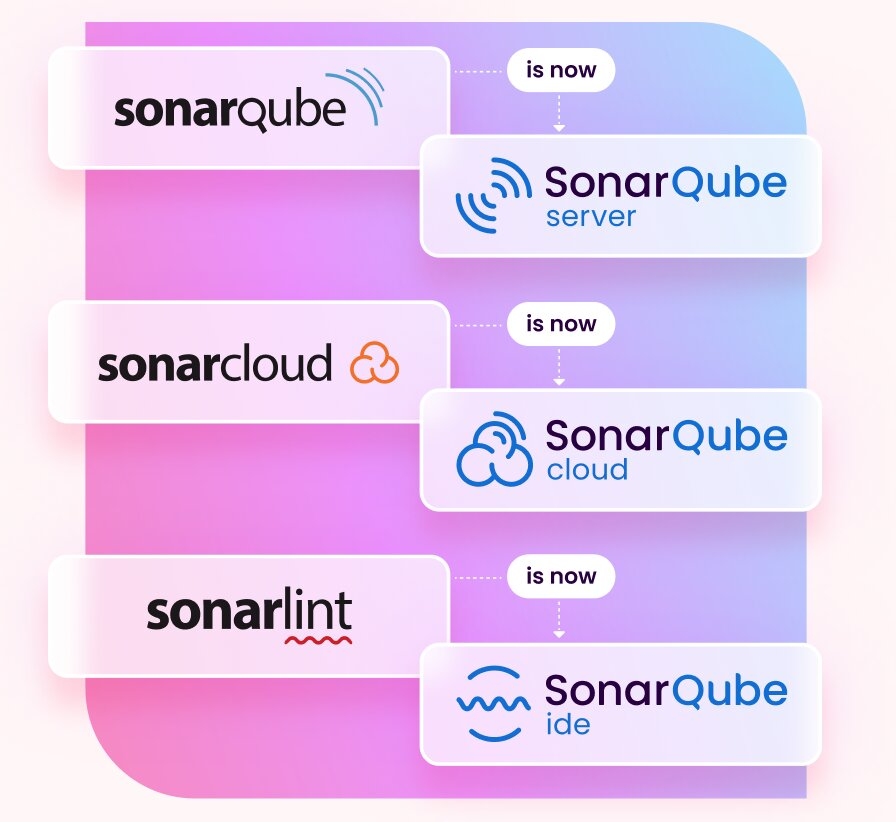
\includegraphics[scale=0.25]{fig/sonar-rebrand-1.jpg}
\end{frame}


\section[Introduction]{Introduction}

\begin{frame}{What is Sonar?}
  
\includegraphics[scale=0.25]{fig/kafka_logo.png}
  \vspace*{2em}
  \begin{itemize}
    \item Open-source \underline{distributed event streaming platform}.
  \end{itemize}
\end{frame}


\section[Why Use SonarCloud?]{Why Use SonarCloud?}

\begin{frame}{Importance of Code Quality}
  % dummy code =============
  \begin{itemize}
    \item Producer
    \item Consumer
    \item Broker
    \item Cluster
    \item Topic
    \item Partitions
    \item Offset
    \item Consumer Groups
    \item Zookeeper
  \end{itemize}
  \begin{tikzpicture}[remember picture, overlay]
    \node[left=3em] at (current page.east)
    {
      
\includegraphics[width=0.35\textwidth]{fig/kafka_logo.png}
    };
  \end{tikzpicture}
  % ============= dummy code 
\end{frame}

\begin{frame}{Security Benefits}
 
\end{frame}

\begin{frame}{Development Best Practices}{Producer}
  \begin{itemize}
    \item A producer is the source of data who will publish events.
  \end{itemize}
  \vspace*{1.5em}
  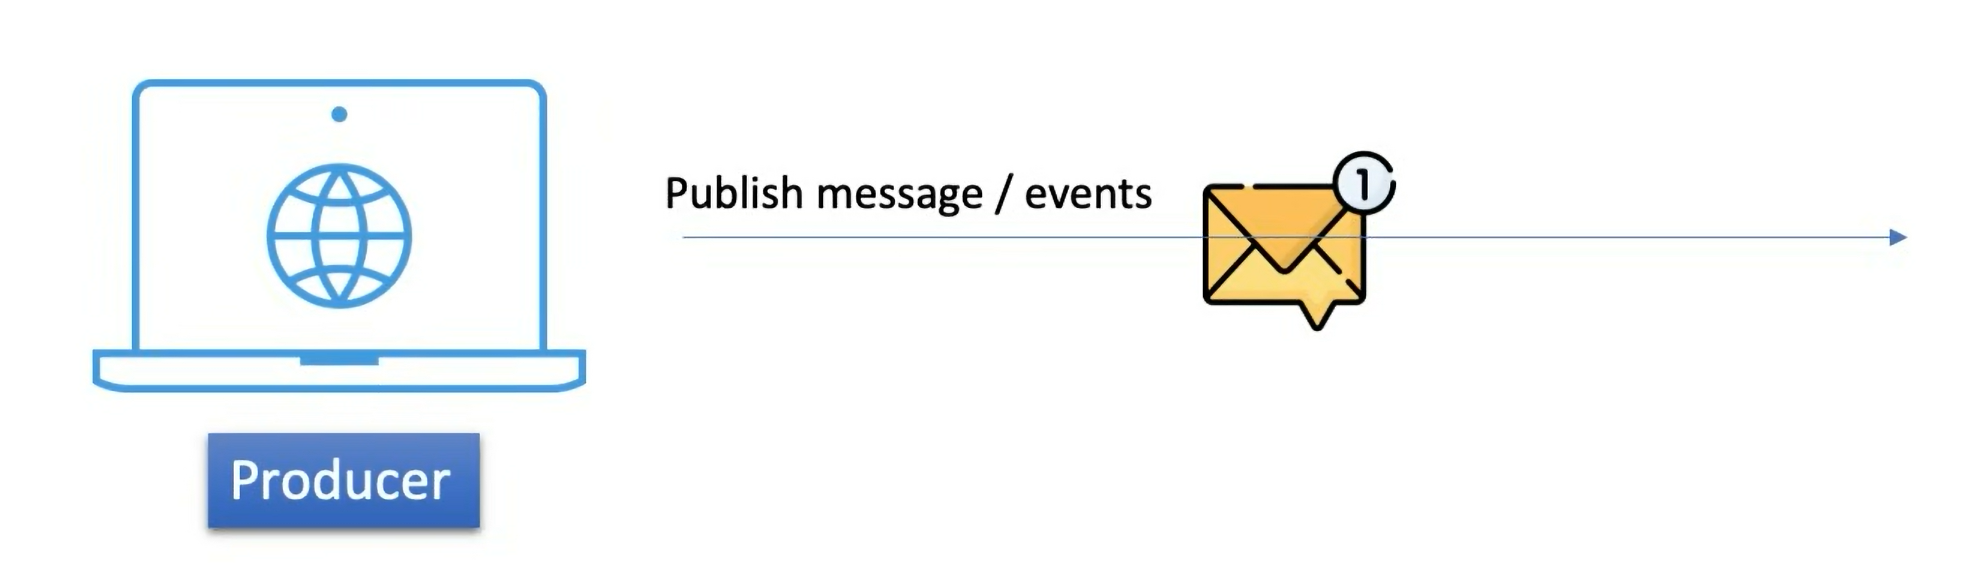
\includegraphics[scale=0.192]{fig/producer.png}
\end{frame}


\section[Key Features]{Key Features}

\begin{frame}{Code Analysis}
  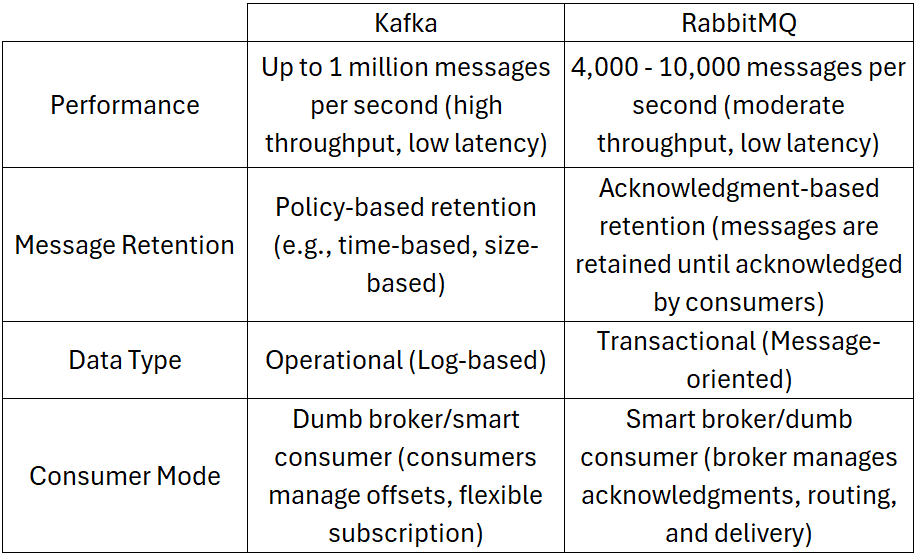
\includegraphics[width=1.02\textwidth]{fig/vs1.png}
\end{frame}

\begin{frame}{Language Support}
  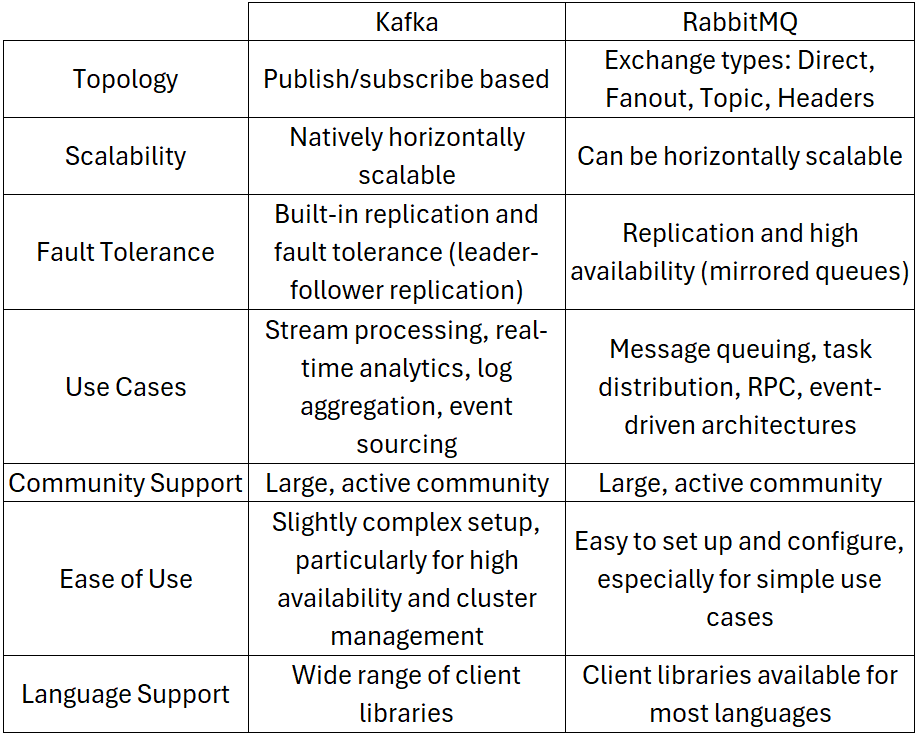
\includegraphics[width=0.99\textwidth]{fig/vs2.png}
\end{frame}

\begin{frame}{Integration Capabilities}
  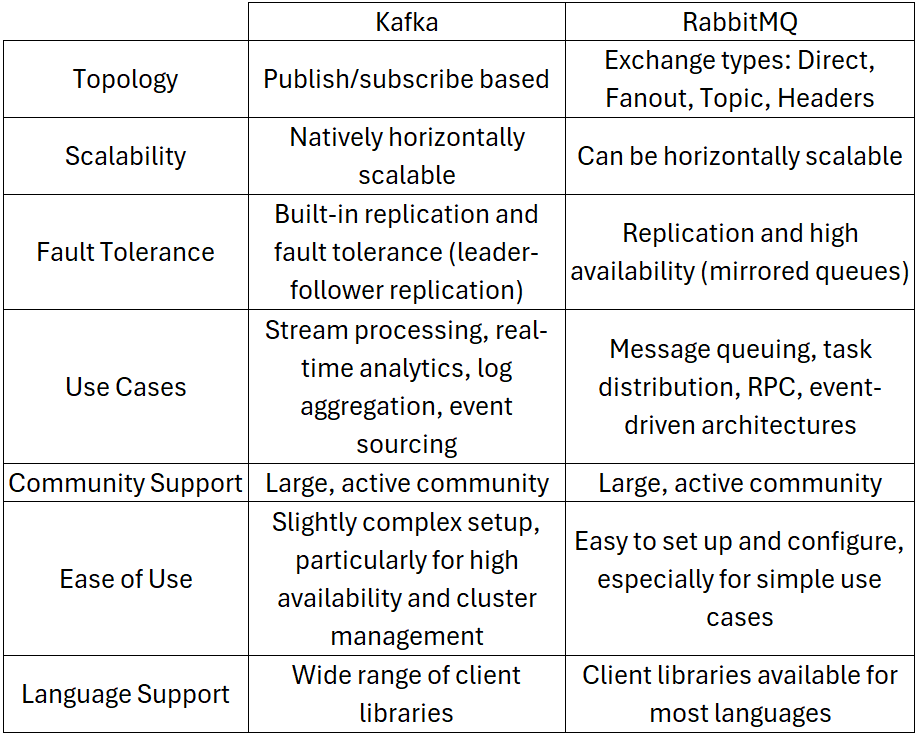
\includegraphics[width=0.99\textwidth]{fig/vs2.png}
\end{frame}

\begin{frame}{Cloud-Based Convenience}
  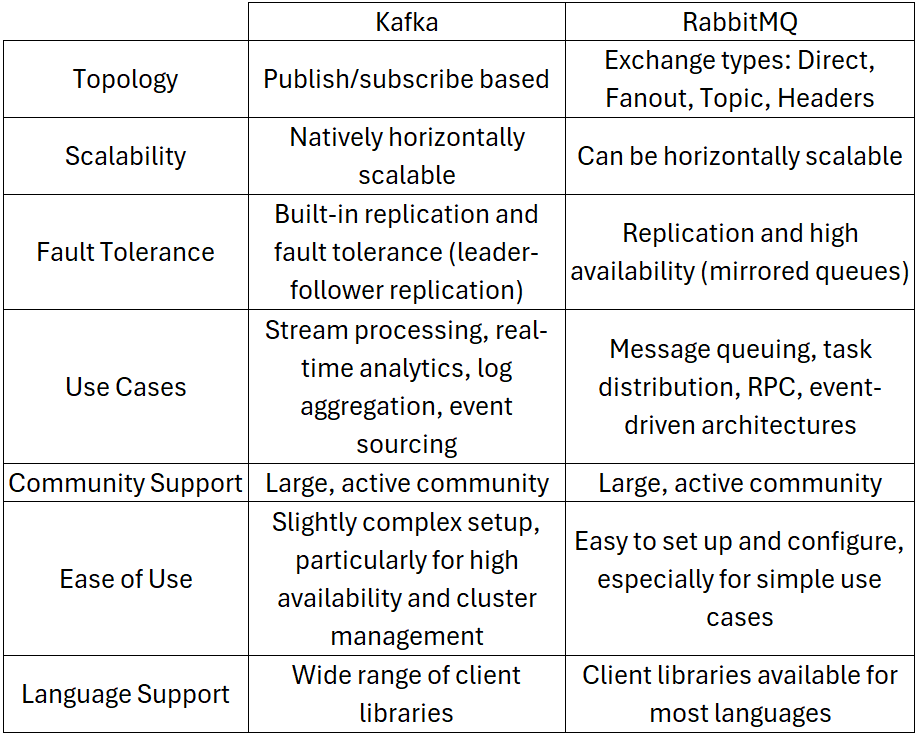
\includegraphics[width=0.99\textwidth]{fig/vs2.png}
\end{frame}


\section[How SonarCloud Works]{How SonarCloud Works}

\begin{frame}{Static Code Analysis}
  \begin{tikzpicture}[remember picture, overlay]
    \node[right=4.02em] at (current page.185)
    {
      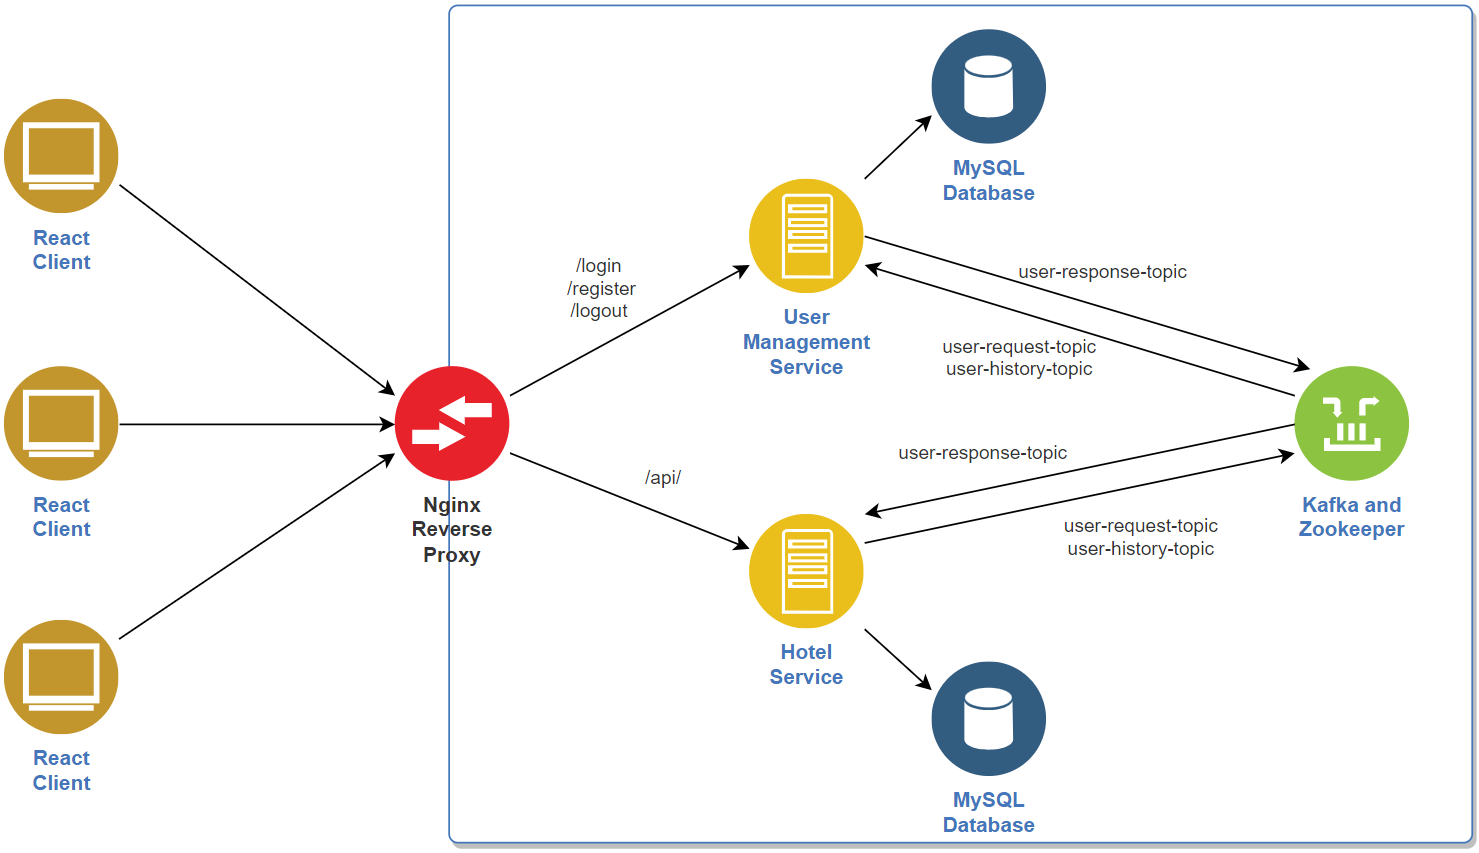
\includegraphics[width=1.09\textwidth]{fig/image.png}
    };
  \end{tikzpicture}
\end{frame}

\begin{frame}{Quality Gates}
 
\end{frame}

\begin{frame}{Dashboard and Reports}
 
\end{frame}


\section[SonarCloud in Action]{SonarCloud in Action}

\begin{frame}{Example Workflow}
 
\end{frame}

\begin{frame}{Live Demo}
 
\end{frame}

\section[ Integration with GitHub and CI/CD Pipelines]{Integration with GitHub and CI/CD Pipelines}

\begin{frame}{Setting Up SonarCloud in GitHub}
 
\end{frame}

\begin{frame}{Basic Pipeline Configuration}
 
\end{frame}


\end{document}
